\documentclass[12pt,a4paper,onecolumn,twoside]{article}

\usepackage{vmargin, xspace}

\usepackage{url}
\usepackage[english]{babel}

\usepackage[absolute]{textpos}
\usepackage{setspace}

\usepackage{amsmath,amssymb}
\usepackage{graphicx,subfigure}
\usepackage{hhline}
\usepackage{arydshln}
\usepackage{myacronym}
\usepackage{multirow}

% My adapted version of pythonlisting
\usepackage{color}
\usepackage[procnames]{listings}
\usepackage{textcomp}
\usepackage{setspace}
\usepackage{palatino}
\renewcommand{\lstlistlistingname}{Code Listings}
\renewcommand{\lstlistingname}{Code Listing}
\definecolor{gray}{gray}{0.5}
\definecolor{green}{rgb}{0,0.5,0}
\definecolor{lightgreen}{rgb}{0,0.7,0}
\definecolor{purple}{rgb}{0.5,0,0.5}
\definecolor{darkred}{rgb}{0.5,0,0}
\definecolor{orange}{rgb}{1,0.5,0}
%\lstnewenvironment{python}[1][]{
%\lstset{
%numbers=left,
%numberstyle=\sffamily\scriptsize,
%numberblanklines=false,
%showstringspaces=false,
%language=python,
%basicstyle=\ttfamily\small\setstretch{1},
%stringstyle=\color{green},
%showstringspaces=false,
%alsoletter={1234567890},
%otherkeywords={\ , \}, \{},
%keywordstyle=\color{blue},
%emph={access,and,as,break,class,continue,def,del,elif,else,%
%except,exec,finally,for,from,global,if,import,in,is,%
%lambda,not,or,pass,print,raise,return,try,while,assert},
%emphstyle=\color{orange}\bfseries,
%emph={[2]self},
%emphstyle=[2]\color{gray},
%emph={[4]ArithmeticError,AssertionError,AttributeError,BaseException,%
%DeprecationWarning,EOFError,Ellipsis,EnvironmentError,Exception,%
%False,FloatingPointError,FutureWarning,GeneratorExit,IOError,%
%ImportError,ImportWarning,IndentationError,IndexError,KeyError,%
%KeyboardInterrupt,LookupError,MemoryError,NameError,None,%
%NotImplemented,NotImplementedError,OSError,OverflowError,%
%PendingDeprecationWarning,ReferenceError,RuntimeError,RuntimeWarning,%
%StandardError,StopIteration,SyntaxError,SyntaxWarning,SystemError,%
%SystemExit,TabError,True,TypeError,UnboundLocalError,UnicodeDecodeError,%
%UnicodeEncodeError,UnicodeError,UnicodeTranslateError,UnicodeWarning,%
%UserWarning,ValueError,Warning,ZeroDivisionError,abs,all,any,apply,%
%basestring,bool,buffer,callable,chr,classmethod,cmp,coerce,compile,%
%complex,copyright,credits,delattr,dict,dir,divmod,enumerate,eval,%
%execfile,exit,file,filter,float,frozenset,getattr,globals,hasattr,%
%hash,help,hex,id,input,int,intern,isinstance,issubclass,iter,len,%
%license,list,locals,long,map,max,min,object,oct,open,ord,pow,property,%
%quit,range,raw_input,reduce,reload,repr,reversed,round,set,setattr,%
%slice,sorted,staticmethod,str,sum,super,tuple,type,unichr,unicode,%
%vars,xrange,zip},
%emphstyle=[4]\color{purple}\bfseries,
%upquote=true,
%morecomment=[s][\color{lightgreen}]{"""}{"""},
%commentstyle=\color{red}\slshape,
%literate={>>>}{\textbf{\textcolor{darkred}{>{>}>}}}3%
%         {...}{{\textcolor{gray}{...}}}3,
%procnamekeys={def,class},
%procnamestyle=\color{blue}\textbf,
%framexleftmargin=1mm, framextopmargin=1mm, frame=shadowbox,
%rulesepcolor=\color{blue},#1
%}}{}

% Initialise the listing settings
\lstset{
numbers=left,
numberstyle=\sffamily\scriptsize,
numberblanklines=false,
showstringspaces=false,
language=python,
basicstyle=\ttfamily\footnotesize\setstretch{1},
stringstyle=\color{green},
showstringspaces=false,
alsoletter={1234567890},
otherkeywords={\ , \}, \{},
keywordstyle=\color{blue},
emph={access,and,as,break,class,continue,def,del,elif,else,%
except,exec,finally,for,from,global,if,import,in,is,%
lambda,not,or,pass,print,raise,return,try,while,assert},
emphstyle=\color{orange}\bfseries,
emph={[2]self},
emphstyle=[2]\color{gray},
emph={[4]ArithmeticError,AssertionError,AttributeError,BaseException,%
DeprecationWarning,EOFError,Ellipsis,EnvironmentError,Exception,%
False,FloatingPointError,FutureWarning,GeneratorExit,IOError,%
ImportError,ImportWarning,IndentationError,IndexError,KeyError,%
KeyboardInterrupt,LookupError,MemoryError,NameError,None,%
NotImplemented,NotImplementedError,OSError,OverflowError,%
PendingDeprecationWarning,ReferenceError,RuntimeError,RuntimeWarning,%
StandardError,StopIteration,SyntaxError,SyntaxWarning,SystemError,%
SystemExit,TabError,True,TypeError,UnboundLocalError,UnicodeDecodeError,%
UnicodeEncodeError,UnicodeError,UnicodeTranslateError,UnicodeWarning,%
UserWarning,ValueError,Warning,ZeroDivisionError,abs,all,any,apply,%
basestring,bool,buffer,callable,chr,classmethod,cmp,coerce,compile,%
complex,copyright,credits,delattr,dict,dir,divmod,enumerate,eval,%
execfile,exit,file,filter,float,frozenset,getattr,globals,hasattr,%
hash,help,hex,id,input,int,intern,isinstance,issubclass,iter,len,%
license,list,locals,long,map,max,min,object,oct,open,ord,pow,property,%
quit,range,raw_input,reduce,reload,repr,reversed,round,set,setattr,%
slice,sorted,staticmethod,str,sum,super,tuple,type,unichr,unicode,%
vars,xrange,zip},
emphstyle=[4]\color{purple}\bfseries,
upquote=true,
morecomment=[s][\color{lightgreen}]{"""}{"""},
commentstyle=\color{red}\slshape,
literate={>>>}{\textbf{\textcolor{darkred}{>{>}>}}}3%
         {...}{{\textcolor{gray}{...}}}3,
procnamekeys={def,class},
procnamestyle=\color{blue}\textbf,
framexleftmargin=1mm, framextopmargin=1mm, frame=shadowbox,
rulesepcolor=\color{blue}
}
\usepackage{comment}

\newcommand{\eqnref}[1]{\eqref{#1}}

\newcommand{\scnref}[1]{section \ref{#1}}
\newcommand{\Scnref}[1]{Section \ref{#1}}

\newcommand{\sbsref}[1]{\S \ref{#1}}
\newcommand{\Sbsref}[1]{Section \ref{#1}}

\newcommand{\figref}[1]{figure \ref{#1}}
\newcommand{\Figref}[1]{Figure \ref{#1}}

\newcommand{\tabref}[1]{Table \ref{#1}}
\newcommand{\Tabref}[1]{Table \ref{#1}}

\newcommand{\twosubs}[2]{\begin{matrix} \\[-14pt] \scriptstyle #1 \\[-3pt] \scriptstyle #2 \end{matrix}} 

% Examples path (added by IRD 14/4/2011)
\newcommand{\dippypath}[0]{C:/COIN}

\begin{document}

\begin{titlepage}
\ 
\setlength{\TPHorizModule}{1cm}
\setlength{\TPVertModule}{1cm}
\begin{textblock}{8.79}(8.655,11.5)
\begin{center}
\textbf{
\begin{Large}
\begin{onehalfspace}
Dippy -- a simplified interface\\[-6pt] for advanced mixed-integer \\[-6pt] programming\\[3pt]
\end{onehalfspace}
\end{Large}
By Dr Michael O'Sullivan, Dr Cameron Walker, Qi-Shan Lim, Dr Stuart Mitchell and Assoc Prof Ted Ralphs\\[3pt]
April 2014\\
%Report, University of Auckland Faculty of Engineering, no. 685 \\
Report, University of Auckland Faculty of Engineering, no. ??? \\
%ISSN 1179-528X % Print version
ISSN 1178-3680 % Electronic version
}
\end{center}
\end{textblock}
\vfill
\end{titlepage}

\title{
Dippy -- a simplified interface for advanced mixed-integer programming
}

%for single author (just remove % characters)
\author{
{\rm Michael O'Sullivan, Qi-Shan Lim and Cameron Walker}\\
Department of Engineering Science, University of Auckland
\and
{\rm Stu Mitchell}\\
Stuart Mitchell Consultants
{\rm Ted Ralphs}\\
Department of Industrial Engineering, Lehigh University
% copy the following lines to add more authors
% \and
% {\rm Name}\\
%Name Institution
} % end author

\date{\today}

\maketitle

\acrodef{MILP}{mixed-integer linear programming}
\acrodef{DIP}{Decomposition for Integer Programming}
\acrodef{CGL}{Cut Generator Library}
\acrodef{OSI}{Open Solver Interface}
\acrodef{DP}{dynamic programming}
\acrodef{TSP}{travelling salesperson}

\subsection*{Abstract}
The development of mathematical modelling languages such as AMPL, GAMS, Xpress-MP and OPL Studio have made it easier to formulate mathematical models such as linear programmes, mixed-integer linear programmes and non-linear programmes for solution in solvers such as CPLEX, MINOS and Gurobi. However, some models cannot be solved using ``out-of-the-box'' solvers, so advanced techniques need to be added to the solver framework.

Many solvers, including CPLEX, Symphony and DIP, provide callback functions to enable users to customise the overall solution framework. However, this approach involves either expressing the mathematical formulation in a low level language such as C++ or Java, or implementing a complicated indexing scheme to be able to track formulation components such as variables and constraints between the mathematical modelling language and the solver's callback framework.

In this paper we present Dippy, a combination of the Python mathematical modelling language PuLP and the open source solver DIP. Using Dippy, users can express their model in a straightforward modelling language and use callback functions to access the PuLP model directly. We discuss the link between PuLP and DIP and give examples of advanced solving techniques expressed simply in Dippy.


\section{Introduction} \label{scn:intro}
Using a high-level modelling language such as AMPL, GAMS, Xpress-MP or OPL Studio enables Operations Research practitioners to express complicated \ac{MILP} problems quickly and (reasonably) easily. Once defined in one of these high-level languages, the \ac{MILP} problem can be solved using one of a number of solvers. However, for many \ac{MILP} problems using solvers ``out of the box'' is only effective for small problem instances (due to the fact that \ac{MILP} problems are NP-hard). Advanced \ac{MILP} techniques are needed for large problem instances and, in many cases, problem-specific techniques need to be included in the solution process.

Both commercial solvers such as CPLEX and open source solvers such as Cbc, Symphony and \acs{DIP} (all from the COIN-OR repository \cite{coin_or}) provide callback functions that allow user-defined routines to be included in the solution framework. However, to make use of the callback functions and develop the user-defined routines, the user must first create their \ac{MILP} problem in a low-level language (C, C++ or Java for Cplex, C or C++ for Cbc, Symphony or \acs{DIP}). While defining their problem, they need to create structures to keep track of appropriate constraints and/or variables for later use in their user-defined routines. For a \ac{MILP} problem of any reasonable size and/or complexity, the problem definition in C/C++/Java is a major undertaking and, thus, a major barrier to the development of customised \ac{MILP} frameworks by both practitioners and researchers.

Given the difficulty of defining a \ac{MILP} problem in a low-level language, another alternative is to return to the high-level mathematical modelling languages (AMPL, GAMS, Xpress-MP, OPL Studio) or their open source equivalents (such as FLOPC++, GAMSlinks and PuLP) to define the \ac{MILP} problem. Then, by carefully constructing an indexing scheme, constraints and/or variables in the high-level language can be identified in the low-level callback functions and advanced \ac{MILP} techniques used. However, implementing the indexing scheme is possibly as difficult as simply using the low-level language to define the \ac{MILP} problem in the first place and so combining high-level and low-level languages does not remove the barrier to solution development.

The purpose of the research presented here is the removal of the barrier that prevents easy experimentation with/customisation of advanced \ac{MILP} solution frameworks. To achieve this aim we need to:
\begin{enumerate}
\item provide an straightforward modelling system so that users can quickly and easily describe their \ac{MILP} problems;
\item enable the callback functions to easily identify constraints and variables in the solution framework.
\end{enumerate}
PuLP already provides a straightforward modelling system for describing \ac{MILP} problems. In our research we extended PuLP so that a \ac{MILP} could be defined and solved using \ac{DIP} \cite{decomp04} within a Python file. We also extended \ac{DIP} so that routines defined within that Python file will be called by the \ac{DIP} callback functions. Variable scope within Python means that these user-defined (Python) routines have complete knowledge of the original problem defined in PuLP. Any extra information required to generate cuts, determine branches or generate columns is provided by the \ac{DIP} callback functions. This ``glue'' between PuLP and \ac{DIP} overcomes the barrier to easy customisation of \ac{DIP} and provides both practitioners and students a straightforward interface for describing problems and customising their solution framework.

The rest of this article is structured as follows. In \scnref{scn:overview} we provide an overview of the interface between PuLP and \ac{DIP}, including a description of the callback functions available in Python from \ac{DIP}. Then, \scnref{scn:define} contains the description and model definition for case studies we will use to demonstrate the effectiveness of Dippy for experimenting with advanced \ac{MILP} techniques. Next, in sections \ref{scn:branch}-\ref{scn:heuristics} we describe how to customise the \ac{DIP} framework to experiment with improvements to the \ac{MILP} solution frameworks available in \ac{DIP}.We conclude in \scnref{scn:concl} where we discuss how this project enhances the ability of researchers to experiment with approaches for solving difficult \ac{MILP} problems.


\section{Combining \ac{DIP} and PuLP} \label{scn:overview}
PuLP is a mathematical modelling language in Python. Using PuLP, a user can quickly and (reasonably) easily define a \ac{MILP} problem and solve it using a variety of solvers including CPLEX, Gurobi and Cbc. As PuLP is built from Python objects it is relatively easy to extend PuLP to use other solvers such as \ac{DIP}. For more details on PuLP see the PuLP project in the COIN-OR repository \cite{coin_or}.

\acf{DIP} \cite{decomp04} provides a framework for solving \ac{MILP} problems using 3 different methods\footnote{The skeleton for a fourth method (branch, relax and cut) exists in \ac{DIP}, but this method is not yet implemented.}: 1) branch and cut; 2) branch, price and cut; and 3) branch, decompose and cut. In this paper we will restrict our attention to 1) and 2).

Branch and cut uses the classic branch-and-bound approach for \ac{MILP} combined with the cutting plane method for removing fractionality in the branch-and-bound nodes' linear programmes. This framework is the basis of many state-of-the-art \ac{MILP} solvers including Gurobi and Cbc. \ac{DIP} provides callback functions for generating user-defined cuts and checking the feasibility of a solution (with respect to the user-defined cuts) within branch and cut. \ac{DIP} also provides a callback function for running a heuristic at each node of the branch-and-bound tree.

Branch, price and cut uses Dantzig-Wolfe decomposition to split a large \ac{MILP} problem into a master problem and one or more subproblems. Branch and cut is used on the master problem. The subproblems solve a pricing problem, defined using the master problem dual values, to add new variables to the master problem.

For branch, price and cut, the cut generation and heuristic callback functions can be used, but extra callback functions enable the user to define their own routines for finding initial variables to include in the master problem and for solving the subproblems to generate new master problem variables. For details on the methods and callback functions provided by \ac{DIP} see \cite{decomp04}.

Dippy extends PuLP to use the \ac{DIP} solver, but it also enables the user-defined routines accessed by the \ac{DIP} callback functions to be implemented in the same Python file as the \ac{MILP} model. Variable scope in Python means that any constraints or variables defined in the \ac{MILP} model are easily accessible in the user-defined routines. Also, \ac{DIP} is implemented so that the \ac{MILP} problem is defined the same way whether branch and cut or branch, price and cut is being used, i.e., it hides the implementation of the master problem and subproblems. This makes it very easy to switch between methods when experimenting with solution methods.

In addition to the \ac{DIP} callback functions (listed in \sbsref{sbs:callbacks}), we have added another callback function that enables user-defined branching in \ac{DIP} and so can be used in any of the solution methods within \ac{DIP}.

\subsection{Callback Functions} \label{sbs:callbacks}

\paragraph{Advanced Branching}
We modified \texttt{chooseBranchVar} in the \ac{DIP} source to become \\ \texttt{chooseBranchSet}. This makes it possible for the user to define:
\begin{itemize}
\item a {\it down} set of variables with (lower and upper) bounds that will be enforced in the down node of the branch; and,
\item an {\it up} set of variables with bounds that will be enforced in the up node of the branch.
\end{itemize}
A typical variable branch on an integer variable $x$ with integer bounds $l$ and $u$ and fractional value $\alpha$ can be implemented by:
\begin{enumerate}
\item choosing the down set to be $\{ x \}$ with bounds $l$ and $\lfloor \alpha \rfloor$;
\item choosing the up set to be $\{ x \}$ with bounds of $\lceil \alpha \rceil$ and $u$.
\end{enumerate}
However, other branching methods may use advanced branching techniques such as the one demonstrated in \scnref{scn:branch}. From \ac{DIP}, {\tt chooseBranchSet} calls \\ {\tt branch\_method} in Dippy.

\paragraph{Customised Cuts} We extended {\tt generateCuts} (in the \ac{DIP} source) to call \\ {\tt generate\_cuts} in Dippy. This enables the user to examine a solution and generate any customised cuts as necessary. We also modified {\tt APPisUserFeasible} to call {\tt is\_solution\_feasible} in Dippy, enabling users to check solutions for feasibility with respect to customised cuts.

\paragraph{Customised Columns (Solutions to Subproblems)} We extended \\ {\tt solveRelaxed} (in \ac{DIP}) to call {\tt relaxed\_solver} in Dippy. This enables the user to utilise the master problem dual variables to produce solutions to subproblems (i.e., columns in the master problem) using customised methods. We also modified {\tt generateInitVars} to call {\tt init\_vars} in Dippy, enabling users to customise the generation of initial columns for the master problem.

\paragraph{Heuristics} We extended {\tt APPheuristics} (\ac{DIP}) to call {\tt heuristics} (Dippy). This enables the user to define customised heuristics at each node in the branch-and-bound tree (including the root node).

\subsection{Interface}

The interface between Dippy (in Python) and DIP (in C++) is summarised in \figref{fig:interface}.
\begin{figure}[htp]
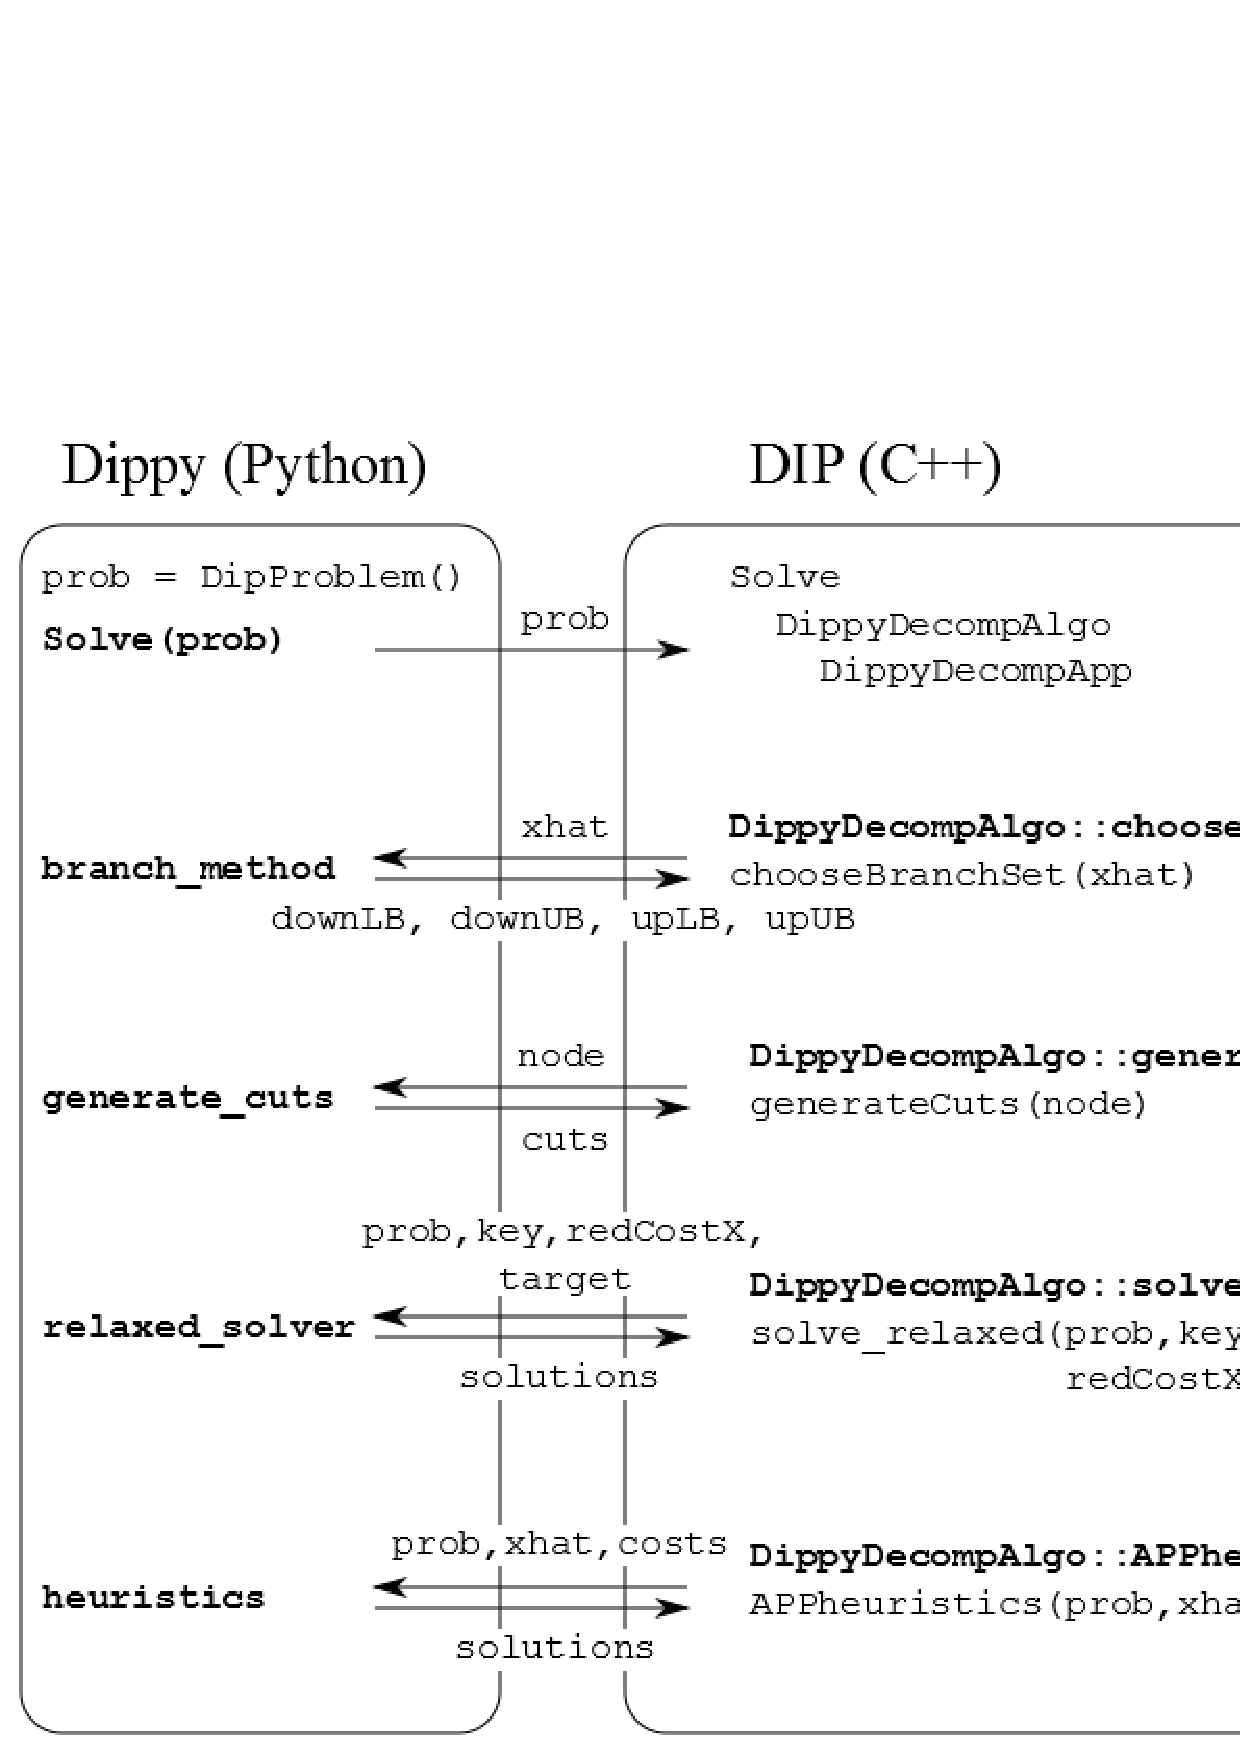
\includegraphics[bb=0 0 960 720,scale=0.45]{interface.png}
\caption{Interface between Dippy and DIP} \label{fig:interface}
\end{figure}

The \ac{MILP} is defined as a {\tt DipProblem} and then solved using the {\tt solve} command in Dippy, that passes the Python {\tt DipProblem} object, {\tt prob}, to DIP in C++. The DIP {\tt solve} creates a {\tt DippyDecompAlgo} object that contains a {\tt DippyDecompApp} object, both of which are populated by data from {\tt prob}. As the DIP {\tt solve} proceeds branches are created by the {\tt DippyDecompAlgo} object using {\tt chooseBranchSet} which passes the current node's fractional solution {\tt xhat} back to the {\tt DipProblem} object {\tt prob}'s {\tt branch\_method} function. This function generates lower and upper bounds for the ``down'' and ``up'' branches and returns to {\tt DippyDecompAlgo::chooseBranchSet}. When DIP generates cuts, it uses the {\tt DippyDecompApp} object's {\tt generateCuts} function which passes the current node's solution {\tt sol} to {\tt prob}'s {\tt generate\_cuts} function. This function generates any customised cuts and returns a list of {\tt cuts} back to \\ {\tt DippyDecompApp::generateCuts}. These interfaces are replicated for the other callback functions provided by Dippy.


\section{Getting Started with Dippy}

*** Put citation info for DIP and Dippy here, make it easy to get 4 citations: DIP paper, DIP software, Dippy paper (this one until journal article is ``born'' and Dippy software ***

\subsection{Installing Dippy} \label{sbs:install}

\subsection{Visualising Search Trees} \label{sbs:gimpy}


\section{Case Studies} \label{scn:define}
In this section we consider the case studies used to demonstrate the use of Dippy. The case studies are:
\begin{enumerate}
\item the bin packing problem;
\item the coke supply chain problem (a capacitated facility location problem within a transshipment problem);
\item the travelling salesperson problem;
\item the cutting stock problem;
\item the wedding planner problem (a set partitioning problem)
\end{enumerate}

In this section we will define the case studies in PuLP and demonstrate their solution in \ac{DIP} without any customisation.  Note that performance metrics throughout this paper were generated using Python 2.6.5 on a Dell Precision M4300 laptop with Intel Core 2 Duo CPU T9500@2.60GHz chipset and 777MHz, 3.50GB of RAM unless otherwise indicated. We used \ac{DIP} version 0.8.7 and Dippy version 1.0.8.

\subsection{The Bin Packing Problem (bin\_pack\_func.py)} \label{sbs:binpack}

The solution of the bin packing problem determines where, amongst $m$ ``bins'', to place $n$ ``items'' of various ``sizes'' in a way that (in this case study) minimises the wasted ``capacity'' of the bins. Each product $j=1, \ldots, n$ has a size $s_j$ and each bin has capacity $C$. Extensions of this problem arise often in \ac{MILP} in problems including network design and rostering.

The \ac{MILP} formulation of the bin packing problem is straightforward. The decision variables are
\begin{align*}
x_{ij} &= \begin{cases} 1 & \text{if item $j$ is placed in bin $i$} \\
0 & \text{otherwise} \end{cases} \\
y_i &= \begin{cases} 1 & \text{if a facility is located at location $i$} \\
0 & \text{otherwise} \end{cases} \\
w_i &= \text{ ``wasted'' capacity at location $i$}
\end{align*}
and the formulation is
\[
\begin{array}{rr@{\ }ll}
       \min & \displaystyle \sum_{i=1}^m w_i \\
\text{s.t.} & \displaystyle \sum_{i=1}^m x_{ij}           & = 1, j = 1, \ldots, n      & \text{ (each product produced)} \\
            & \displaystyle \sum_{j=1}^n r_j x_{ij} + w_i & = C y_i, i = 1, \ldots, m  & \text{ (aggregate capacity at location $i$)} \\
            & \multicolumn{2}{l}{x_{ij} \leq y_i, i = 1, \ldots, m, j = 1, \ldots, n}  & \text{ (disaggregate capacity at location $i$)} \\[6pt]
            & \multicolumn{3}{l}{x_{ij} \in \{ 0, 1\}, w_i \geq 0, y_i \in \{0, 1\}, i = 1, \ldots, m, j = 1, \ldots, n}
\end{array}
\]

Note that the disaggregate capacity constraints are not necessary for defining the solution, but tighten the \ac{MILP} formulation ( i.e., remove factional solutions from the solution space). Using PuLP we can easily define this \ac{MILP} problemm in Dippy. The entire input file is given below with a summary for each fragment.

\begin{enumerate}
\item Load PuLP and Dippy;
\lstinputlisting[linerange=3-20]{../../examples/Dippy/bpp/bin_pack_func.py}

\item Get the problem data from another file. This determines $j=1, \ldots, n$, $i = 1, \ldots, m$, $r_j, j = 1, \ldots, n$ and $C$;
\lstinputlisting[firstnumber=9,linerange=9-10]{C:/COIN/Dip/Dip/examples/Dippy/bpp/bin_pack_func.py}
For {\tt facility\_ex1.py} $n = 5, m = 5, r = (7, 5, 3, 2, 2)^\top$ and $C = 8$.

\item Define the \ac{MILP} problem and the problem variables;
\lstinputlisting[firstnumber=15,linerange=15-24]{../../examples/Dippy/bpp/bin_pack_func.py}

\item Define the objective function;
\lstinputlisting[firstnumber=26,linerange=26-27]{../../examples/Dippy/bpp/bin_pack_func.py}

\item Define the constraints; \lstinputlisting[firstnumber=29,linerange=29-42]{../../examples/Dippy/bpp/bin_pack_func.py}

\item Solve the \ac{MILP} problem using \ac{DIP} using default options except for a user-defined zero tolerance and then display the solution;
\lstinputlisting[firstnumber=235,linerange=235-244]{../../examples/Dippy/bpp/bin_pack_func.py}
\end{enumerate}
Running the preceding Python codes takes 1.17s of CPU time, creates a tree with 375 nodes and gives the following output
\begin{verbatim}
Location  1  produces  [1]
Location  4  produces  [4, 5]
Location  5  produces  [2, 3]
\end{verbatim}

Note that \ac{DIP} uses cuts from the \ac{CGL} \cite{coin_or} by default. We can turn all cuts off by setting the {\tt generateCuts} flag to 0 and turn \ac{CGL} cuts off by setting the {\tt CutCGL} flag to 0. We will use these settings to explore the effect of user-defined cuts in \scnref{scn:cuts}.


\subsection{The Coke Supply Chain Problem (coke.py)} \label{sbs:coke}

This case study is sourced from the Operations Research Web in the Department of Engineering Science TWiki \cite{coke} (and was originally adapted from Leyland et al. \cite{geoff_coke}). There are 6 coal mines that produce coal. The coal is transported from the 6 mines to a coke-making plant where it is converted to coke using ``thermal decomposition''. Every tonne of coke produced by thermal decomposition requires 1.3 tonnes of coal. From the coke-making plants the coke is transported to one of 6 customers. There are 6 locations where coke-making plants can be constructed. There are 6 different size plants that can be constructed at each location.

The size of a plant determines the coke processing level in kilotonnes/year the plant can produce. \Tabref{tab:plant_size} shows the different plant sizes with their corresponding processing levels and construction cost in million RMB.
\begin{table}[htp]
\begin{center}
\begin{tabular}{|c|c|c|}
\hline
\multirow{2}{*}{\bf Plant Size} & {\bf Processing Level} & {\bf Cost} \\
 & {\bf (kT/year)} & {\bf (MRMB)} \\
\hline
1 & 75 & 4.4 \\
2 & 150 & 7.4 \\
3 & 225 & 10.5 \\
4 & 300 & 13.5 \\
5 & 375 & 16.5 \\
6 & 450 & 19.6 \\
\hline
\end{tabular}
\caption{Possible plant sizes} \label{tab:plant_size}
\end{center}
\end{table}

To get this problem into Dippy we use the PuLP modelling language. The entire input file is given below with a summary for each fragment.

\begin{enumerate}
\item Load PuLP and Dippy;
\lstinputlisting[firstnumber=5,linerange=5-6]{../../examples/coke.py}

\item Define the coke-from-coal conversion rate and a big-$M$ variable for use in later constraints;
\lstinputlisting[firstnumber=8,linerange=8-9]{C:/COIN/Dippy/examples/coke.py}

\item Define the supply of coal at the mines, the possible locations and construction costs of the coke-making plants and the demand for coke from the customers.
\lstinputlisting[firstnumber=11,linerange=11-22]{../../examples/coke.py}
\newpage
\lstinputlisting[firstnumber=24,linerange=24-45]{../../examples/coke.py}

\item Define the transportation costs from the mines to the coke-making plants and the coke-making plants to the customers in two tables (we also define a function {\tt read\_table} to read these tables, but this function is omitted for brevity);
\lstinputlisting[firstnumber=47,linerange=47-65]{../../examples/coke.py}

\item Read the data from the tables;
\lstinputlisting[firstnumber=79,linerange=79-81]{../../examples/coke.py}

\item Define the arcs and their costs from the mine $\rightarrow$ plant and plant $\rightarrow$ customer costs;
\lstinputlisting[firstnumber=83,linerange=83-86]{../../examples/coke.py}

\item \label{itm:2d} Define a 2-dimensional set for the plant sizes at each location;
\lstinputlisting[firstnumber=88,linerange=88-89]{../../examples/coke.py}

\item Create a \texttt{DipProblem} (extended from \texttt{LpProblem} in PuLP). Add binary variables that determine the plant sizes at each location and (non-negative) integer variables that determine the flow (in coal from the mines to the plants and coke from the plants to the customers) transported through the network;
\lstinputlisting[firstnumber=91,linerange=91-99]{../../examples/coke/coke.py}

\item Add the objective of minimising total cost = building costs (converted from MRMB to RMB) + transportation costs;
\lstinputlisting[firstnumber=101,linerange=101-106]{../../examples/coke.py}

\item Add constraints that limit the flow of coke out of a coke-making plant depending on the capacity plant constructed;
\lstinputlisting[firstnumber=108,linerange=108-113]{../../examples/coke.py}

\item Add constraints that limit the number of coke-making plants built at any single location to be one (Note. there is a size with capacity 0 if no plant will be built);
\lstinputlisting[firstnumber=115,linerange=115-118]{../../examples/coke.py}

\item Add constraints to conserve flow at the mines ($\leq$ supply), coke-making plants (flow in = coke-from-coal conversion rate $\times$ flow out) and customers ($\geq$ demand);
\lstinputlisting[firstnumber=120,linerange=120-133]{../../examples/coke.py}

\item Solve the \ac{MILP} problem using \ac{DIP} and display the solution in tabular form;
\lstinputlisting[firstnumber=160,linerange=160-178]{../../examples/coke.py}
\end{enumerate}

The preceding Python code defines and solves the Coke Supply Chain Problem. The solution takes 1.09s of CPU time and creates a tree using 201 nodes. The output defines plants to be built at locations 1, 5 and 6 and also defines shipments of coal and coke between the mines, plants and customers:
\begin{verbatim}
Build L1 150 (1.0)
Build L2 0 (1.0)
Build L3 0 (1.0)
Build L4 0 (1.0)
Build L5 450 (1.0)
Build L6 300 (1.0)

        L1       L2      L3      L4      L5      L6
M1      0.0      0.0     0.0     0.0     0.0     25.8
M2      0.0      0.0     0.0     0.0     0.0     340.475
M3      124.1175 0.0     0.0     0.0     585.0   0.0
M4      0.0      0.0     0.0     0.0     0.0     0.0
M5      0.0      0.0     0.0     0.0     0.0     0.0
M6      0.0      0.0     0.0     0.0     0.0     0.0

        C1       C2      C3      C4      C5      C6
L1      83.0     0.0     6.975   0.0     0.0     5.5
L2      0.0      0.0     0.0     0.0     0.0     0.0
L3      0.0      0.0     0.0     0.0     0.0     0.0
L4      0.0      0.0     0.0     0.0     0.0     0.0
L5      0.0      0.0     0.0     0.0     450.0   0.0
L6      0.0      5.5     0.0     5.5     270.75  0.0
\end{verbatim}



\subsection{The Travelling Salesperson Problem (tsp.py)} \label{sbs:tsp}

This case study is a small \acf{TSP} example. This problem differs from the previous case studies (\sbsref{sbs:facility} and \sbsref{sbs:coke}) in that it can't be expressed explicitly for any reasonable size problem. To completely define the \ac{TSP} problem requires a number of subtour elimination constraints that is $O(2^n)$ where $n = |N|$ is the number of locations the salesperson must visit in their tour. The standard way to solve \ac{TSP} problems is to use a formulation without any subtour elimination constraints and dynamically add only the subtour elimination constraints needed to define an optimal tour. Here we will use PuLP to define the \ac{MILP} formulation without subtour elimination constraints.

\begin{enumerate}
\item Load PuLP, Dippy and the square root function from the math module;
\lstinputlisting[linerange=1-3]{../../examples/Dippy/tsp/tsp.py}

\newpage

\item Define the cities and their locations in the $xy$-plane. Also, define empty structures for arcs between each pair of cities and int/out of cities;
\lstinputlisting[firstnumber=7,linerange=7-17]{../../examples/Dippy/tsp/tsp.py}

\item Define the Euclidean distance using {\tt sqrt};
\lstinputlisting[firstnumber=19,linerange=19-21]{../../examples/Dippy/tsp/tsp.py}

\item Define the arcs between cities, the arcs in/out of a city and the cost of the arcs as the distance between cities;
\lstinputlisting[firstnumber=21,linerange=23-31]{../../examples/Dippy/tsp/tsp.py}

\item Use the standard \ac{TSP} \ac{MILP} formulation without any subtour constraints. The standard formulation is:
\begin{align*}
\min & \sum_{(i, j) \in A} c_{ij} x_{ij} \\
     & \sum_{\twosubs{(i, j) \in A}{i = k \text{ or } j = k}} x_{ij} = 2, k \in N.
\end{align*}
\lstinputlisting[firstnumber=33,linerange=33-38]{../../examples/Dippy/tsp/tsp.py}
\lstinputlisting[firstnumber=40,linerange=40-42]{../../examples/Dippy/tsp/tsp.py}

\item  Solve the \ac{TSP} using \ac{DIP} and display the minimum cost tour;
\lstinputlisting[firstnumber=118,linerange=118-124]{../../examples/Dippy/tsp/tsp.py}

\end{enumerate}

Solving the \ac{TSP} using \ac{DIP} takes 0.13s of CPU time and gives the following solution:
\begin{verbatim}
(5, 9) 1.0
(4, 7) 1.0
(1, 3) 1.0
(4, 8) 1.0
(5, 6) 1.0
(6, 9) 1.0
(2, 3) 1.0
(0, 1) 1.0
(7, 8) 1.0
(0, 2) 1.0
\end{verbatim}
with 3 subtours:
\begin{enumerate}
\item $0 \rightarrow 1 \rightarrow 3 \rightarrow 2 \rightarrow 0$;
\item $4 \rightarrow 7 \rightarrow 8 \rightarrow 4$;
\item $5 \rightarrow 6 \rightarrow 9 \rightarrow 5$.
\end{enumerate}

The optimal \ac{TSP} solution can only be found by adding user-defined cuts that remove subtours. \Scnref{scn:cuts} describes how to implement these user-defined cuts in Dippy and shows how these cuts combine with the \ac{CGL} cuts to efficiently solve this \ac{TSP}.


\subsection{The Cutting Stock Problem (cutting\_stock.py)} \label{sbs:sponge}

This case study also come from the Operations Research Web in the Department of Engineering Science TWiki \cite{sponge}. The solution of this problem defines cutting patterns to produce the required demand for items from standard items. In this case study the demand is for variable length sponge rolls to be cut from standard length rolls. The entire input file is given below with a summary for each fragment.

\begin{enumerate}
\item Load PuLP and Dippy;
\lstinputlisting[linerange=1-2]{../../examples/Dippy/csp/cutting_stock.py}

\item Define the length of sponge rolls required and the demand for each length of sponge roll (note, some variations of demand are shown but have been commented out);
\lstinputlisting[firstnumber=4,linerange=4-8]{../../examples/Dippy/csp/cutting_stock.py}
\lstinputlisting[firstnumber=10,linerange=10-22]{../../examples/Dippy/csp/cutting_stock.py}

\item Define the maximum number of possible patterns used for cutting the standard rolls (at most one standard roll for each sponge roll needed) and the length of the standard rolls;
\lstinputlisting[firstnumber=24,linerange=24-29]{../../examples/Dippy/csp/cutting_stock.py}

\item Define a two dimensional set of items cut from patterns (cf. \ref{itm:2d} from \sbsref{sbs:coke});
\lstinputlisting[firstnumber=31,linerange=31-32]{../../examples/Dippy/csp/cutting_stock.py}

\newpage

\item Create a \texttt{DipProblem}. Add binary variables that determine if each pattern is used and (non-negative, bounded) integer variables that define the number of sponge rolls of each length cut from a particular pattern.
\lstinputlisting[firstnumber=34,linerange=34-40]{../../examples/Dippy/csp/cutting_stock.py}
Note that normally we would define an integer variable that defines how many times a pattern is used and, thus, need less patterns. However, \ac{DIP} does not (yet) solve identical subproblems simultaneously, so we need one subproblem for each pattern cut;

\item We want to minimise the total number of standard rolls used;
\lstinputlisting[firstnumber=42,linerange=42-43]{../../examples/Dippy/csp/cutting_stock.py}

\item We want to meet demand for sponge rolls;
\lstinputlisting[firstnumber=45,linerange=45-48]{../../examples/Dippy/csp/cutting_stock.py}

\item Add constraints that make sure patterns are used ``in order'' (these constraints are not strictly necessary but remove symmetry in the solution space);
\lstinputlisting[firstnumber=50,linerange=50-53]{../../examples/Dippy/csp/cutting_stock.py}

\item Create one subproblem for each pattern that makes sure the sponge rolls cut from the standard roll in the pattern do not exceed the length of the standard roll. Note the \texttt{relaxation[p]} on line 57. This adds the constraint to the Dantzig-Wolfe subproblem if branch, price and cut is used (for more details see \scnref{scn:cuts});
\lstinputlisting[firstnumber=55,linerange=55-59]{../../examples/Dippy/csp/cutting_stock.py}

\item Solve the Sponge Roll Production Problem using branch, price and cut.  Display the patterns used and the sponge rolls cut from those patterns. Note that the \texttt{doPriceCut} options is turned on (set to 1). This means that \ac{DIP} will use branch, price and cut instead of branch and cut;
\lstinputlisting[firstnumber=186,linerange=186-198]{../../examples/Dippy/csp/cutting_stock.py}

\end{enumerate}

This problem takes 33.31s of CPU time and requires 175 nodes in the branch-and-bound tree for the master problem. The solution uses 2 standard rolls cut as follows:
\begin{itemize}
\item Standard roll 0: 2 $\times$ 5cm rolls and 1 $\times$ 9cm roll = 19cm used (1cm wasted);
\item Standard roll 1: 2 $\times$ 5cm rolls and 1 $\times$ 7cm roll = 17cm used (3cm wasted).
\end{itemize}


\subsection{The Wedding Planner Problem (wedding.py)} \label{sbs:wedding}

This case study is taken from the PuLP documentation \cite{pulp}. Given a list of wedding attendees, a wedding planner must come up with a seating plan to minimise the unhappiness of all of the guests. The unhappiness of guest is defined as their maximum unhappiness at being seated with each of the other guests at their table, i.e., it is a pairwise function. The unhappiness of a table is the maximum unhappiness of all the guests at the table. All guests must be seated and there is a limited number of seats at each table.

The wedding planner problem is a set partitioning problem. The set of guests $G$ must be partitioned into multiple subsets, with each subset seated at the same table. The cardinality of the subsets is determined by the number of seats at a table and the unhappiness of a table can be determined by the subset. The \ac{MILP} formulation is:
\[
\begin{array}{rrl}
& x_{gt} &= \begin{cases} 1 & \text{if guest $g$ sits at table $t$} \\
 0 & \text{otherwise} \end{cases} \\
& u_t &= \text{unhappiness of table $t$} \\
& S &= \text{number of seats at a table} \\
& U(g, h) &= \text{unhappiness of guests $g$ and $h$ if they are seated at the same table}
\end{array}
\]\[
\begin{array}{rrl}
\min & \displaystyle \sum_{t \in T} u_t & \text{(total unhappiness of the tables)} \\
& \displaystyle \sum_{g \in G} x_{gt} &\leq S, t \in T \\
& \displaystyle \sum_{t \in T} x_{gt} &=1, g \in G \\
& u_t &\geq U(g, h) (x_{gt} + x_{ht} - 1), t \in T, g < h \in G
\end{array}
\]

To get this problem into Dippy we use the PuLP modelling language. The entire model follows with a summary for each fragment:
\begin{enumerate}
\item Load PuLP and Dippy;
\lstinputlisting[firstnumber=8,linerange=8-9]{../../examples/Dippy/wedding/wedding.py}

\item Define the unhappiness function for the guests (in this case we use letters in the alphabet as guests and the ``distance'' between two letters in the guest list as their unhappiness at being seated together);
\lstinputlisting[firstnumber=15,linerange=15-20]{../../examples/Dippy/wedding/wedding.py}

\item Get the problem data from an external program  (this is used to test various inputs to the \ac{MILP} formulation);
\lstinputlisting[firstnumber=22,linerange=22-22]{../../examples/Dippy/wedding/wedding.py}

\item Create a the \texttt{DipProblem} for Dippy;
\lstinputlisting[firstnumber=26,linerange=26-27]{../../examples/Dippy/wedding/wedding.py}

\item Create a set for the tables and also for all possible seatings, i.e., pairs $g \in G, t \in T$;
\lstinputlisting[firstnumber=29,linerange=29-34]{../../examples/Dippy/wedding/wedding.py}

\newpage

\item Create the seating variables $x_{gt}, g \in G, t \in T$;
\lstinputlisting[firstnumber=36,linerange=36-42]{../../examples/Dippy/wedding/wedding.py}

\item Create the table unhappiness variables $u_t, t \in T$;
\lstinputlisting[firstnumber=44,linerange=44-48]{../../examples/Dippy/wedding/wedding.py}

\item Create the objective that minimises the total unhappiness of the tables;
\lstinputlisting[firstnumber=50,linerange=50-51]{../../examples/Dippy/wedding/wedding.py}

\item Create the constraints for: 1) the number of seats at a table; 2) ensuring each guest is seated; and 3) defining table unhappiness;
\lstinputlisting[firstnumber=53,linerange=53-57]{../../examples/Dippy/wedding/wedding.py}
\lstinputlisting[firstnumber=59,linerange=59-75]{../../examples/Dippy/wedding/wedding.py}

\newpage

\item Solve the problem using branch, price and cut;
\lstinputlisting[firstnumber=157,linerange=157-159]{../../examples/Dippy/wedding/wedding.py}

\end{enumerate}

Note the \texttt{relaxation[table]} syntax on lines 55 and 72. This defines a separate subproblem for each table that contains the constraint for the number of seats at a table and the constraints defining table unhappiness. These table subproblems are used in branch, price and cut.

For a simple example, where the wedding guests are \{ A, B, C, D, E, F, G, H, I, J, K \}, the solution time is 1.28s of CPU time and the tree consists of 1395 nodes. The solution is
\begin{verbatim}
Table 0 = ['D', 'E', 'F', 'G']
Table 1 = ['A', 'B', 'C']
Table 2 = ['H', 'I', 'J', 'K']
\end{verbatim}



\section{Adding Customised Branching} \label{scn:branch}
In \scnref{sbs:callbacks} we explained the modifications to \ac{DIP} (\texttt{chooseBranchVar} to \\ \texttt{chooseBranchSet}) and also how to implement a simple variable branch using \texttt{chooseBranchSet}. However, other branching methods may use advanced branching techniques such as the ones demonstrated in the remainder of this section.

From \ac{DIP}, \texttt{chooseBranchSet} calls \texttt{branch\_method} in Dippy. In Dippy, we can implement customised branching by defining a \texttt{branch\_method}. The function \texttt{branch\_method} has two inputs supplied by \ac{DIP}:
\begin{enumerate}
\item \texttt{prob} -- the \texttt{DipProblem} being solved;
\item \texttt{sol} -- an indexable object representing the solution at the current node.
\end{enumerate}
We define \texttt{branch\_method} using these inputs in the same Python file as the model definition. Note that Dippy can access the variables from the original formulation. Due to Python's scoping rules, no complicated indexing or searching is required (also note Python starts its array indexing at 0 -- cf. C/C++).

\subsection{Advanced Branching in the Capacitated Facility Location problem} \label{sbs:fac_brch}

When solving the facility location problem (see \sbsref{sbs:facility}) one difficulty is symmetry in the solution space. Since the facilities are identical, solvers consider multiple solutions that differ only in the labelling of the facility locations. To overcome this constraints for ordering the facility locations can be included:
\[ y_i \geq y_{i+1}, i = 1, \ldots, m-1 \]
\lstinputlisting[firstnumber=44,linerange=44-47]{C:/COIN/Dippy/examples/facility.py}

These ordering constraints also introduce the opportunity to implement an effective branch on the number of facilities. If $\displaystyle\sum_{i=1}^m y_i = \alpha \notin \mathbb{Z}$, then:
\vspace*{-6pt}
\begin{center}
\begin{tabular}{l|l}
the branch down restricts & the branch up restricts \\
$\displaystyle\sum_{i=1}^m y_i \leq \lfloor \alpha \rfloor$ &
$\displaystyle\sum_{i=1}^m y_i \geq \lceil \alpha \rceil$ \\
and the ordering means that & and the ordering means that \\
$y_i = 0, i = \lceil \alpha \rceil, \ldots, m$ &
$y_i = 1, i = 1, \ldots, \lceil \alpha \rceil$
\end{tabular}
\end{center}

To implement this branch in Dippy simply requires the definition of the \\ \texttt{branch\_method}. Remember Python's scoping rules allow the model structures to be accessed directly within our customised branching function, no complicated indexing or searching is necessary.
\lstinputlisting[firstnumber=49,linerange=49-65]{C:/COIN/Dippy/examples/facility.py}

By only adding the ordering constraints we improve the solution time from 1.17s to 0.28s of CPU time and decrease the tree size from 375 to 76 nodes. By adding the advanced branching we decrease the solution time further to 0.05s of CPU time and the tree size decreases to 3 nodes. A full summary of the effect of advanced \ac{MILP} methods, including branching is given in \scnref{scn:concl}.

\subsection{Advanced Branching in the Coke Supply Chain problem}

In the Coke Supply Chain problem, the main source of fractionality is the size of the plant facilities. If the necessary size to process coal to coke is between the given sizes then the \texttt{buildVars} variable will be fractional. We can define a branch that forces the plant to be either less than the nearest given size below or greater than the nearest given size above. For example, if the size = 210, then it lies between the given sizes of 150 and 225, so the branch down keeps the size $\leq$ 150 and the branch up keeps the size $\geq$ 225. However, branching on the size of the plant itself does not help reduce fractionality as the fractional amounts simply change to match the new plant size. The most effective way to enforce the branch and reduce fractionality is by banning infeasible variables. In our example, in the down branch all buildVars for the location with capacity $>$ 150 are set to 0 (by setting the upper bound to 0) and in the up branch all buildVars for the location with capacity $<$ 255 are set to 0 (also by setting the upper bound to 0). We can define this branching in Dippy.
\lstinputlisting[firstnumber=135,linerange=135-158]{C:/COIN/Dippy/examples/coke.py}

With this advanced branching the solution time decreases from 1.09s to 0.62s of CPU time and the tree reduces from 201 nodes to 76 nodes.

\begin{comment}

\subsection{Advanced Branching in the Wedding Planner problem} \label{sbs:wed_brch}

When solving the Wedding Planner problem using \ac{MILP}, guests will often be ``split'' between tables. Branching a particular $x_{gt}$ to 0 is not effective as linear programming can simply swap entire tables and maintain the split on a different table. One way to strengthen branching if some $x_{gt}$ is fractional is to: 1) find the minimum index table $t$ with $x_{gt} > 0$; 2) define a ``down'' branch that restricts guest $g$ to sit at tables with index $t$ or smaller; 3) define a ``up'' branch that restricts guest $g$ to sit at tables with index $t + 1$ or bigger. This method creates more balanced branches and reduces the size of the branch-and-bound tree.
\lstinputlisting[firstnumber=77,linerange=77-90]{C:/COIN/Dippy/examples/wedding_dip.py}

With this advanced branching the solution times get worse and the tree size increases! Not a good branch...

\end{comment}




\section{Adding Customised Cut Generation} \label{scn:cuts}
\acrodef{CGL}{Cut Generation Library}
\begin{sloppypar} By default \ac{DIP} uses the \ac{CGL} to add cuts. We can use \lstinline{dippyOpts} to turn off \ac{CGL} cuts and observe how effective the \ac{CGL} are
\lstinputlisting[firstnumber=73,linerange={107-108,110-110,115-117}]{../../examples/Dippy/bpp/bin_pack_func.py}
The branch-and-bound tree is significantly larger (see figure \ref{fig:bpp_tree4}) than the original branch-and-bound tree that only used \ac{CGL} cuts (see figure \ref{fig:bpp_tree1}).
\begin{figure}[htp]
\begin{center}
\includegraphics[scale=0.075]{img/bpp_tree4.eps}
\end{center}
\caption{Branch-and-bound tree for bin packing problem instance without \ac{CGL} cuts.} \label{fig:bpp_tree4}
\end{figure}


To add user-defined cuts in Dippy, we first define a new procedure for generating cuts and (if necessary) a procedure for determining a feasible solution.
Within Dippy, this requires two new functions, \lstinline{generate_cuts} and \lstinline{is_solution_feasible}.
As in \sbsref{sbs:branch}, the embedded bin packing problem and decisions variables make it easy to access the solution values of variables in the bin packing problem.
The inputs to \lstinline{is_solution_feasible} are:
\begin{enumerate}
\item \lstinline{prob} -- the \lstinline{DipProblem} being solved;
\item \lstinline{sol} -- an indexable object representing the solution at the current node;
\item \lstinline{tol} -- the zero tolerance value.
\end{enumerate}
and the inputs to \lstinline{generate_cuts} are:
\begin{enumerate}
\item \lstinline{prob} -- the \lstinline{DipProblem} being solved;
\item \lstinline{node} -- various properties of the current node, including the solution.
\end{enumerate}

If a solution is determined to be infeasible either by \ac{DIP} (for example some integer variables are fractional) or by \lstinline{is_solution_feasible} (which is useful for solving problems like the travelling salesman problem with cutting plane methods), cuts will be generated by \lstinline{generate_cuts} and the in-built \ac{CGL} (if enabled).\end{sloppypar}

\begin{comment}

Marchand and Wolsey \cite{agg_mir2001} define many types of cuts for \ac{MILP} problems.
One of these is the \textit{weighted inequality}.
For each facility location $i$ and some subset $S_i (\subseteq \{1, \ldots, n \})$ of the products we can calculate
\[ \mu_i = C - \sum_{j \in S_i} w_j x_{ij} \]
and use it to generate a weighted inequality
\[ \sum_{j \in S_i} w_j x_{ij} + \sum_{j \notin S_i} (w_j - \mu_i)^+ x_{ij} \leq C - \mu _i \]
which forms a valid inequality for the facility location problem.

The cut generating function creates the subsets $S_i$ for each location from the fractional solution in a greedy way depending on the $x_{ij}$ values, and from these we generate a set of weighted inequality cuts.
The code listing below shows how to build the set of cuts, and omits the generation of $S_i$ for the sake of brevity.
\lstinputlisting[firstnumber=67,linerange=67-74]{../../examples/Dippy/bpp/bin_pack_func.py}
$\vdots$\newpage
\lstinputlisting[firstnumber=98,linerange=98-111]{../../examples/Dippy/bpp/bin_pack_func.py}

Adding the weighted inequality cut generator reduces the branch-and-bound tree size from 419 nodes to 77 nodes.

\end{comment}

\section{Adding Customised Column Generation} \label{scn:column}
Using Dippy it is easy to transform a problem into a form that can be solved by either branch-and-cut or branch-price-and-cut.
Branch-price-and-cut decomposes a problem into a master problem and a number of distinct subproblems.
We can identify subproblems using the \lstinline{relaxation} member of the \lstinline{DipProblem} class.
Once the subproblems have been identified, then they can either be ignored (when using branch-and-cut -- the default method for \ac{DIP}) or utilised (when using branch-price-and-cut -- specified by turning on the \lstinline{doPriceCut} option).

In branch-price-and-cut, the original problem is decomposed into a master problem and multiple subproblems~\cite{DWDecomp00}:
\begin{equation}
\begin{array}{rr@{\ }r@{\ }r@{\ }r@{\ }l}
             \min & c_1^\top x_1 & + \ c_2^\top x_2 & + \ \cdots & + \ c_K^\top x_K \\
\text{subject to} & A_1 x_1      & + \ A_2 x_2      & + \ \cdots & + \ A_K x_K      & = b \\
                  &              &   F_2 x_2      &          &                & = f_2 \\
                  &              &                &  \ddots  &                & \ \ \vdots \\
                  &              &                &          &   F_K x_K      & = f_K \\
                  & x_1 \in \mathbb{Z}^{+}_{n_1} &, x_2 \in \mathbb{Z}^{+}_{n_2}&, \ldots, x_K & \in \mathbb{Z}^{+}_{n_K} \quad
\end{array}
\label{eqn:decomp}
\end{equation}

In \eqref{eqn:decomp}, there are $K-1$ subproblems defined by the constraints $F_k x_k = f_k, k \in 2, \ldots, K$. The constraints $A_1 x_1 + A_2 x_2 + \cdots + A_K x_K = b$ are known as \textit{linking} constraints. Instead of solving \eqref{eqn:decomp} directly, column generation uses a convex combination of solutions $y^k$ to each subproblem $j$ to define the subproblem variables:
\begin{equation}
x_k = \sum_{l_k=1}^{L_k} \lambda^k_{l_k} y^k_{l_k} \label{eqn:combin}
\end{equation}
where $0 \leq \lambda^k_{l_k} \leq 1$ and $\sum_{l_k=1}^{L_k} \lambda^k_{l_k} = 1$. By substituting \eqref{eqn:combin} into the linking constraints and recognising that each $y^k_{l_k}$ satisfies $F_k x_k = f_k, x_k \in \mathbb{Z}^{+}_{n_k}$ (as it is a solution of this subproblem), we can form the \textit{restricted} master problem (RMP) with corresponding duals ($\pi$, $\gamma_1, \ldots, \gamma_K$):
\begin{equation}
\begin{array}{rr@{\ }r@{\ }r@{\ }r@{\ }ll}
             \min & c_1^\top x_1 & + \displaystyle\sum_{l_2=1}^{L_2} \left(c_2^\top y^2_{l_2} \right) \lambda^2_{l_2} & + \ \cdots & + \displaystyle\sum_{l_K=1}^{L_K} \left(c_K^\top y^K_{l_K} \right) \lambda^K_{l_K} \\
\text{subject to} & A_1 x_1      & + \displaystyle\sum_{l_2=1}^{L_2} \left(A_2 y^2_{l_2} \right) \lambda^2_{l_2} & + \ \cdots & + \displaystyle\sum_{l_K=1}^{L_K} \left( A_K y^K_{l_K} \right) \lambda^K_{l_K}      & = b & : \pi \\
                  &              &   \displaystyle\sum_{l_2=1}^{L_2} \lambda^2_{l_2}      &          &                & = 1 & : \gamma_1 \\
                  &              &                &  \ddots  &                & \ \ \vdots \\
                  &              &                &          &   \displaystyle\sum_{l_K=1}^{L_K} \lambda^K_{l_K}      & = 1 & : \gamma_K \\
                  &              &   \displaystyle\sum_{l_2=1}^{L_2} y^2_{l_2} \lambda^2_{l_2}      &          &                & \in \mathbb{Z}^{+}_{n_2} \\
                  &              &                &  \ddots  &                & \ \ \vdots \\
                  &              &                &          &   \displaystyle\sum_{l_K=1}^{L_K} y^K_{l_K} \lambda^K_{l_K}      & \in \mathbb{Z}^{+}_{n_K} \\
                  &          x_1 & \in \mathbb{Z}^{+}_{n_1}, \lambda^2 \in [0, 1]_{L_2}, & \ldots, \lambda^K & \in [0, 1]_{L_K} \hspace{1.25cm} &
\end{array}
\label{eqn:rmp}
\end{equation}
The RMP provides the optimal solution $x^*_1, x^*_2, \ldots, x^*_K$ to the original problem \eqref{eqn:decomp} if the necessary subproblem solutions are present in the RMP. That is, if $y^{k,*}_{l_k}, l_k =1, \ldots, L_k, k = 2, \ldots K$ such that $x^*_k = \sum_{l_k=1}^{L_k} \lambda^k_{l_k} y^{k,*}_{l_k}, k = 2, \ldots, K$ have been included.

Given that $x^*_k, k = 1, \ldots, K$ are not known a priori, column generation starts with an initial solution consisting of $x_1$ and initial sets of subproblem solutions. ``Useful'' subproblem solutions, that form columns for the RMP, are found by looking for subproblem solutions that provide columns with negative reduced cost. The reduced cost of a solution $y^k_{l_k}$'s column, i.e., the reduced cost for $\lambda^k_{l_k}$,  is given by $c_k^\top y^k_{l_k} - \pi^\top A_k y^k_{l_k} - \gamma_k$. To find a solution with minimum reduced cost we can solve:
\begin{equation}
\begin{array}{rr@{\,}ll}
{\cal S}_k: \min & (c_k - \pi^\top A_k)^\top &x_k - \gamma_k & \text{(reduced cost for corresponding $\lambda^k$)} \\
\text{subject to} & F_k & x_k      = f_k & \text{(ensures that $y^k$ solves subproblem $k$)} \\
                  & & x_k \in \mathbb{Z}^{+}_{n_k}
\end{array}
\label{eqn:subprob}
\end{equation}
If the objective value of ${\cal S}_k$ is less than $0$, then the solution $y^k$ will form a column in the RMP whose inclusion in the basis would improve the objective value of the RMP. The solution $y^k$ is added to the set of solution used in the RMP. There are other mechanisms for managing the sets of solutions present in \ac{DIP}, but they are beyond the scope of this paper.

Within \ac{DIP}, hence Dippy, the RMP and \textit{relaxed} problems $S_k, k = 2, \ldots, K$ are not specified explicitly. Rather, the constraints for each subproblem $F_k x_k = f_k$ are specified by using the \lstinline{.relaxation[j]} syntax. \ac{DIP} then automatically constructs the RMP and the relaxed problems $S_k, k = 2, \ldots, K$. The relaxed subproblems $S_k, k = 2, \ldots, K$ can either be solved using the default \ac{MILP} solver (CBC) or a customised solver. A customised solver can be defined by the \lstinline{relaxed_solver} function.
This function has 4 inputs:
\begin{enumerate}
\item \lstinline{prob} -- the \lstinline{DipProblem} being solved;
\item \lstinline{index} -- the index $k$ of the subproblem being solved;
\item \lstinline{redCosts} -- the reduced costs for the $x_k$ variables $c_k - \pi^\top A_k$;
\item \lstinline{convexDual} -- the dual value for the convexity constraint for this subproblem $\gamma_k$.
\end{enumerate}
In addition to subproblem solutions generated using RMP dual values, initial columns for subproblems can also be generated either automatically using CBC or using a customised approach.
A customised approach to initial variable generation can be defined by the \lstinline{init_vars} function.
This function has only 1 input, \lstinline{prob}, the \lstinline{DipProblem} being solved.

Starting from the original capacitated facility location problem from \scnref{scn:techs}:
\[
\begin{array}{rr@{\ }ll}
       \min & \displaystyle \sum_{i=1}^m w_i \\
\text{s.t.} & \displaystyle \sum_{i=1}^m x_{ij}           & = 1, j = 1, \ldots, n      & \text{ (each product produced)} \\
            & \displaystyle \sum_{j=1}^n r_j x_{ij} + w_i & = C y_i, i = 1, \ldots, m  & \text{ (aggregate capacity at location $i$)} \\
            & \multicolumn{2}{l}{x_{ij} \leq y_i, i = 1, \ldots, m, j = 1, \ldots, n}  & \text{ (disaggregate capacity at location $i$)} \\[6pt]
            & \multicolumn{3}{l}{x_{ij} \in \{ 0, 1\}, w_i \geq 0, y_i \in \{0, 1\}, i = 1, \ldots, m, j = 1, \ldots, n}
\end{array}
\]
we can decompose this formulation:
\[
\begin{array}{r@{\ }r@{\ }r@{\ }r@{\ }c@{\ }r@{\ }l@{\ }l}
%      r           r                 r         r          c             r               l        
\min        &                     &        &  1 w_2 & \cdots &                     &  +1 w_m 				\\
\text{s.t.} & I \mathbf{x}_2      &        &        & \cdots & + I \mathbf{x}_m    &         &= 1 \text{ (each product produced)} \\
            & r^\top \mathbf{x}_2 & -C y_2 & +1 w_2 &        &                     &         &= 0 \text{ (aggregate cap. at loc. 2)} \\
            & I \mathbf{x}_2      & -e y_2 &        &        &                     &         &\leq 0 \text{ (disaggregate cap. at loc. 2)}\\
            &                     &        &        & \ddots \\
            &                     &        &        &        & r^\top \mathbf{x}_m & -C y_m +1 w_m  & = 0 \text{ (aggregate cap. at loc. K)}\\
            &                     &        &        &        & + I \mathbf{x}_m    & -e y_m         & \leq 0 \text{ (disaggregate cap. at loc. K)}
\end{array}
\]
where
\[
\mathbf{x}_i = \begin{pmatrix}
x_{i1} \\ \vdots \\ x_{in}
\end{pmatrix}, r = \begin{pmatrix}
r_{1} \\ \vdots \\ r_{n}
\end{pmatrix} \text{ and }
e = \begin{pmatrix}
1 \\ \vdots \\ 1
\end{pmatrix}.
\]
Now the subproblems $F_k x_k = f_k, k = 2, \ldots, K$ are
\[
\begin{bmatrix}
r^\top & -C & 1 \\
I & e 
\end{bmatrix} \begin{bmatrix}
\mathbf{x}_i \\
y_i \\
w_i
\end{bmatrix}
\begin{matrix}
= \\ \leq
\end{matrix}
\begin{bmatrix}
0 \\ 0
\end{bmatrix},
\]
\[ c_k^\top = \left[ \begin{array}{c|c|c} 0 & 0 & 1 \end{array} \right], A_k = \left[ \begin{array}{c|c|c} I & 0 & 0 \end{array} \right], \]
so ${\cal S}_k$ becomes
\[
\begin{array}{rr@{\ }r@{\ }r@{\ }l}
{\cal S}_i: \min  & \sum_{j=1}^n -\pi_j x_{ij} \, &           & +1 w_i & - \gamma_i \\
\text{subject to} & \sum_{j=1}^n r_j    x_{ij} \, & -C y_i \, & +1 w_i & = 0 \\
                  &                     x_{ij} \, & -  y_i \, &        & \leq 0, j = 1, \ldots, n \\
                  &                     x_{ij},   &    y_i,   & \in \{0, 1 \}, & j = 1, \ldots, n, w_i \geq 0
\end{array}
\]
where $\pi_j$ is the dual variable for the assignment constraint for product $j$ in the RMP.

\begin{sloppypar}In Dippy, we define subproblems for each facility location using the \lstinline{.relaxation} syntax for the aggregate and disaggregate capacity constraints:\end{sloppypar}
\lstinputlisting[firstnumber=32,linerange=32-41]{../../examples/Dippy/bpp/bin_pack_decomp_func.py}

All remaining constraints (the assignment constraints that ensure each product is assigned to a facility) form the master problem when using branch-price-and-cut.
To use branch-price-and-cut we turn on the \lstinline{doPriceCut} option:
\lstinputlisting[firstnumber=206,linerange=206-209]{../../examples/Dippy/bpp/bin_pack_decomp_func.py}

Note that symmetry is also present in the decomposed problem, so we add ordering constraints (described in \sbsref{sbs:branch}) to the RMP :
\lstinputlisting[firstnumber=43,linerange=43-46]{../../examples/Dippy/bpp/bin_pack_decomp_func.py}

\begin{sloppypar}Using branch-price-and-cut, the RMP takes about ten times as long to solve as the original formulation, and has a search tree size of 37 nodes.
The \lstinline{generateInitVars} option uses CBC by default to find initial columns for the RMP and then uses CBC to solve the relaxed problems.
Dippy lets us provide our own approaches to solving the relaxed problems and generating initial variables, which may be able to speed up the overall solution process.\end{sloppypar}

In the relaxed problem for location $i$, the objective simplified to $\min \sum_{j=1}^n -\pi_j x_{ij} +1 w_i - \gamma_i$. 
However, the addition of the ordering constraints and the possibility of a Phase I/Phase II approach in the \ac{MILP} solution process to find initial variables mean that our method must work for any reduced costs, i.e., the objective becomes $\min \sum_{j=1}^n d_j x_{ij} + f y_i + g w_i - \gamma_i$. Although the objective changes, the constraints remain the same. If we choose not to use a location, then $x_{ij} = y_i = w_i = 0$ for $j=1, \ldots, n$ and the objective is $-\gamma_i$. Otherwise, we use the location and $y_i = 1$ and add $f$ to the objective. The relaxed problem reduces to:
\[
\begin{array}{rr@{\ }r@{\ }l}
\min              & \sum_{j=1}^n d_j x_{ij} \, & +g w_i & - \gamma_i \\
\text{subject to} & \sum_{j=1}^n r_j x_{ij} \, & +1 w_i & = C \\
                  &                  x_{ij},   &    w_i    & \in \{0, 1 \}, j = 1, \ldots, n
\end{array}
\]
However, the constraint ensures $w_i = C - \sum_{j=1}^n r_j x_{ij}$, so we can reformulate as:
\[
\begin{array}{rr@{\ }l}
\min              & \sum_{j=1}^n (d_j - g r_j) x_{ij} \, & +f C - \gamma_i \\
\text{subject to} & C - \sum_{j=1}^n r_j x_{ij} & \geq 0 \Rightarrow \sum_{j=1}^n r_j x_{ij} \leq C \\
                  &                  x_{ij},   & \in \{0, 1 \}, j = 1, \ldots, n
\end{array}
\]
This is a 0-1 knapsack problem with ``effective costs'' costs for each product $j$ of $d_j - g r_j$. We can use dynamic programming to find the optimal solution.

In Dippy, we can access the problem data, variables and their reduced costs, so the 0-1 knapsack dynamic programming solution is straightforward to implement and use:
\lstinputlisting[firstnumber=66,linerange=66-81]{../../examples/Dippy/bpp/bin_pack_decomp_func.py}
$\vdots$\newpage
\lstinputlisting[firstnumber=83,linerange=83-105]{../../examples/Dippy/bpp/bin_pack_decomp_func.py}

Adding this customised solver reduces the solution time because it has the benefit of knowing it is solving a knapsack problem rather than a general \ac{MILP}.

To generate initial facilities (complete with assigned products) we implemented two approaches.
The first approach used a first-fit method and considered the products in order of decreasing requirement:
\lstinputlisting[firstnumber=146,linerange=146-169]{../../examples/Dippy/bpp/bin_pack_decomp_func.py}
\newpage
\lstinputlisting[firstnumber=172,linerange=172-184]{../../examples/Dippy/bpp/bin_pack_decomp_func.py}
The second approach simply assigned one product to each facility:
\lstinputlisting[firstnumber=186,linerange=186-197]{../../examples/Dippy/bpp/bin_pack_decomp_func.py}

Using Dippy we can define both approaches at once and then define which one to use by setting the \lstinline{init_vars} method:
\lstinputlisting[firstnumber=199,linerange=199-200]{../../examples/Dippy/bpp/bin_pack_decomp_func.py}

These approaches define the initial sets of subproblem solutions $y^k_{l_k}, l_k=1,$ $\ldots, L_k, k = 1, \ldots, K$ for the initial RMP before the relaxed problems are solved using the RMP duals.

The effect of the different combinations of column generation, customised subproblem solvers and initial variable generation methods, both by themselves and combined with branching, heuristics, etc are summarised in \tabref{tab:fac_exp}. For this size of problem, column generation does not reduce the solution time significantly (if at all). However, we show in \scnref{scn:concl} that using column branching enables \ac{DIP} (via Dippy and PuLP) to be competitive with state-of-the-art solvers.

\section{Adding Customised Heuristics} \label{scn:heuristics}
To add user-defined heuristics in Dippy, we first define a new procedure for node heuristics, \texttt{heuristics}. This function has three inputs:
\begin{enumerate}
\item \texttt{prob} -- the \texttt{DipProblem} being solved;
\item \texttt{xhat} -- an indexable object representing the fraction solution at the current node;
\item \texttt{cost} -- the objective coefficients of the variables.
\end{enumerate}
Multiple heuristics can be executed and all heuristic solutions can be returned to \ac{DIP}. Different problems benefit from different heuristic approaches and a heuristic that solves the original problem may not be as useful when a fractional solution is available. We show how solve a heuristic for the overall problem and also how to implement a heuristic for fractional solutions. As in \scnref{scn:branch}, Python's scoping rules allow us to easily access the solution values of variables in our problem.

\subsection{Customised Heuristics for the Capacitated Facility Location problem} \label{sbs:fac_heur}

An initial allocation of production to locations can be found heuristically using the same first-fit heuristic that provided initial solutions for the column generation approach (see \sbsref{sbs:fac_cols}). The first-fit heuristic iterates through the items requiring production and the facility locations allocating production at the first facility that has sufficient capacity to produce the item.
\lstinputlisting[firstnumber=116,linerange=116-127]{C:/COIN/Dippy/examples/facility.py}

\vfill
\newpage
\lstinputlisting[firstnumber=129,linerange=129-144]{C:/COIN/Dippy/examples/facility.py}

The first-fit heuristic can then be used to provide an initial, feasible solution at the root node within the customised \texttt{heuristics} function (see lines 215-220):
\lstinputlisting[firstnumber=211,linerange=211-230]{C:/COIN/Dippy/examples/facility.py}

Running the first-fit heuristic before starting the branching process increases the solution time from 1.17s to 1.48s of CPU time and the number of nodes in the search tree from 375 nodes to 399 nodes.

\newpage

At each node in the branch-and-bound tree, the fractional solution (provided by \texttt{xhat}) gives an indication of the best allocation of production, albeit fractional. One heuristic approach to ``fixing'' the fractional solution is to consider each allocation (of an item's production to a facility) in order of decreasing fractionality and use a first-fit approach:
\lstinputlisting[firstnumber=146,linerange=146-192]{C:/COIN/Dippy/examples/facility.py}
\newpage
\lstinputlisting[firstnumber=194,linerange=194-209]{C:/COIN/Dippy/examples/facility.py}

The first-fit approach that is guided by fractional values can then be used within the \texttt{heuristics} function (see lines 225-229 in the previous listing) to create integer solutions from fractional solutions at each node.

Adding the first-fit heuristic guided by fractional values increases the solution time further from 1.48s to 1.89s of CPU time and the number of nodes remains at 399.

The reason this heuristic (in fact any heuristic) was not that helpful for this problem is that:
\begin{itemize}
\item the optimal solution is found within the first 10 nodes without any heuristics, so the heuristic only provides an improved upper bound for $< 10$ nodes;
\item the extra overhead of the heuristic at each node increases the solution time and the heuristic affects the search procedure in a way that more nodes are explored.
\end{itemize}

Heuristics generally only help in problems where feasibility is more difficult by providing upper bounds when ``fixing'' fractional solutions. In this problem, the optimal solution is found quickly and the rest of the search tree checks solutions that are symmetric.

In \scnref{scn:concl} we show the effect of the heuristic when symmetry is removed.

\begin{comment}
\subsection{Customised Heuristics for the Wedding Planner problem} \label{sbs:wed_heur}
\end{comment}

\section{Conclusions} \label{scn:concl}
In \scnref{scn:techs} we showed how Dippy works in practice by making customisations to the solver framework for an example problem.
We will use the Wedding Planner problem from the PuLP documentation \cite{pulp} to compare Dippy to two leading solvers that utilise branch-and-cut: the open-source CBC and the commercial Gurobi.
This particular problem is useful for comparing performance because it has a natural column generation formulation and can be scaled-up in a simple way, unlike the Facility Location problem which is strongly dependent on the specific instance being tested.

The Wedding Planner problem is as follows: given a list of wedding attendees, a wedding planner must come up with a seating plan to minimise the unhappiness of all of the guests.
The unhappiness of guest is defined as their maximum unhappiness at being seated with each of the other guests at their table, making it a pairwise function.
The unhappiness of a table is the maximum unhappiness of all the guests at the table.
All guests must be seated and there is a limited number of seats at each table.

This is a set partitioning problem, as the set of guests $G$ must be partitioned into multiple subsets, with the members of each subset seated at the same table.
The cardinality of the subsets is determined by the number of seats at a table and the unhappiness of a table can be determined by the subset.
The \ac{MILP} formulation is:
\[
\begin{array}{rrl}
& x_{gt} &= \begin{cases} 1 & \text{if guest $g$ sits at table $t$} \\
 0 & \text{otherwise} \end{cases} \\
& u_t &= \text{unhappiness of table $t$} \\
& S &= \text{number of seats at a table} \\
& U(g, h) &= \text{unhappiness of guests $g$ and $h$ if they are seated at the same table}
\end{array}
\]\[
\begin{array}{rrl}
\min & \displaystyle \sum_{t \in T} u_t & \text{(total unhappiness of the tables)} \\
& \displaystyle \sum_{g \in G} x_{gt} &\leq S, t \in T \\
& \displaystyle \sum_{t \in T} x_{gt} &=1, g \in G \\
& u_t &\geq U(g, h) (x_{gt} + x_{ht} - 1), t \in T, g < h \in G
\end{array}
\]

Since \ac{DIP}, and thus Dippy, doesn't require a problem to be explicitly formulated as a Dantzig-Wolfe decomposition, a change from \ac{DIP} to CBC is trivial.
The only differences are that:
\begin{enumerate}
\item A \lstinline{LpProblem} is created instead of a \lstinline{DipProblem};
\item No \lstinline{.relaxation} statements are used;
\item The \lstinline{LpProblem.solve} method uses CBC to solve the problem.
\end{enumerate}
To see if CBC and Gurobi would perform well with a column-based approach, we also formulated a problem equivalent to the restricted master problem from the branch-price-and-cut approach and generated and added all possible columns before the solving the \ac{MILP}.
Finally we used to Dippy to develop a customised solver and initial variable generation function for the branch-price-and-cut formulation in \ac{DIP}.
In total, six approaches were tested on problem instances of increasing size:
\begin{enumerate}
\item CBC called from PuLP;
\item CBC called from PuLP using a columnwise formulation and generating all columns a priori;
\item Gurobi called from PuLP;
\item Gurobi called from PuLP using a columnwise formulation and generating all columns a priori;
\item \ac{DIP} called from Dippy using branch-price-and-cut without customisation;
\item \ac{DIP} called from Dippy using customised branching, cuts and column generation callback functions.
\end{enumerate}

In \Tabref{tab:wed_exp} and \Figref{fig:compare} we see that\footnote{All tests were run using Python 2.7.1 on a Dell XPS1530 laptop with an Intel Core~2~Duo CPU T9500@2.60GHz and 4~GB of RAM. We used CBC version~2.30.00, Gurobi version~4.5.1, and Dippy version~1.0.10.}:
\begin{itemize}
\item Gurobi is fastest for small problems;
\item The symmetry present in the problem means the solution time of CBC and Gurobi for the original problem deteriorate quickly;
\item The time taken to solve the columnwise formulation also deteriorates, but at a lesser rate than when using CBC or Gurobi on the original problem;
\item Both \ac{DIP} and customised \ac{DIP} solution times grow at a lesser rate than any of the CBC/Gurobi approaches;
\item For large problems, \ac{DIP} becomes the preferred approach.
\end{itemize}

The main motivation for the development of Dippy was to alleviate obstacles to experimentation with and customisation of advanced \ac{MILP} frameworks.
These obstacles arose from an inability to use the description of a problem in a high-level modelling languag integrated with the callback functions in leading solvers.
This is mitigated with Dippy by using the Python-based modelling language PuLP to describe the problem and then exploiting Python's variable scoping rules to implement the callback functions.

Using the Capacitated Facility Location problem we have shown that Dippy is relatively simple to experiment with and customise, enabling the user to quickly and easily test many approaches for a particular problem, including combinations of approaches.
In practice Dippy has been used successfully to enable final year undergraduate students to experiment with advanced branching, cut generation, column generation and root/node heuristics.
%Given the demonstrated ease of the implementation of advanced \ac{MILP} techniques and the flexibility of a high-level mathematical modelling language, the above evidence that Dippy can be highly competitive solver for problems in which column generation is the preferred approach suggests that Dippy is effective as more than just an experimental ``toy'' or educational tool.
The Wedding Planner problem shows that Dippy can be a highly competitive solver for problems in which column generation is the preferred approach.
Given the demonstrated ease of the implementation of advanced \ac{MILP} techniques and the flexibility of a high-level mathematical modelling language, this suggests that Dippy is effective as more than just an experimental ``toy'' or educational tool.
It enables users to concentrate on furthering Operations Research knowledge and solving hard problems instead of spending time worrying about implementation details.
Dippy breaks down the barriers to experimentation with advanced \ac{MILP} approaches for both practitioners and researchers.


\begin{table}[htp]
\begin{minipage}[l]{\textwidth}
\begin{small}
\begin{tabular}{|l@{\,}|c@{\ }|c@{\ }c@{\ }|c@{\ }|c@{\ }c@{\ }|c@{\ }c@{\,}|}
\hline
\textbf{\# guests} & \multicolumn{8}{|c|}{\textbf{Time (s)}} \\
                   & CBC & \multicolumn{2}{c|}{CBC \& columns} & Gurobi & \multicolumn{2}{c|}{Gurobi \& columns} & \ac{DIP} & Customised \\
                   &     & gen vars & solve                    &        & gen vars & solve                       &          & \ac{DIP}   \\ 
\hline 
 6 &  0.07 & 0.01 &   0.06 &   0.04 & 0.01 &   0.05 &   0.90 &  0.33 \\
 7 &  0.07 & 0.01 &   0.12 &   0.04 & 0.01 &   0.11 &   1.77 &  0.57 \\
 8 &  0.90 & 0.01 &   0.27 &   0.07 & 0.01 &   0.25 &   4.78 &  0.57 \\
 9 &  2.54 & 0.01 &   0.57 &   0.09 & 0.01 &   0.55 &   2.11 &  0.78 \\
10 &  3.83 & 0.01 &   1.23 &   0.13 & 0.01 &   1.15 &   5.60 &  0.94 \\
11 &  6.48 & 0.01 &   2.46 &   0.14 & 0.01 &   2.36 &   8.62 &  0.91 \\
12 & 26.73 & 0.01 &   4.64 &   0.34 & 0.01 &   4.55 &  25.17 &  2.80 \\
13 & 53.18 & 0.01 &   8.57 &   0.39 & 0.01 &   8.28 &  14.86 &  1.40 \\
14 & 70.51 & 0.01 &  15.27 &   0.38 & 0.01 &  14.65 &  20.09 &  2.66 \\
15 & 97.79 & 0.01 &  26.26 &   0.47 & 0.01 &  25.07 &  33.52 &  1.59 \\
16 &$>$1000& 0.01 &  43.86 &  68.08 & 0.01 &  42.11 &  26.73 &  2.09 \\
17 &    -- & 0.01 &  72.07 &  79.71 & 0.01 &  68.87 &  50.48 &  3.92 \\
18 &    -- & 0.01 & 115.64 &  96.03 & 0.01 & 110.52 &  40.80 &  4.67 \\
19 &    -- & 0.01 & 181.39 & 113.01 & 0.01 & 173.13 &  78.20 &  2.64 \\
20 &    -- & 0.02 & 283.16 &$>$6000 & 0.01 & 270.08 &  61.86 &  5.31 \\
21 &    -- & 0.02 & 434.60 &     -- & 0.02 & 418.04 &  77.66 &  4.23 \\
22 &    -- & 0.02 & 664.87 &     -- & 0.02 & 639.04 & 134.76 &  4.63 \\
23 &    -- &   -- &$>$1000 &     -- &   -- &$>$1000 & 149.82 &  9.16 \\
24 &    -- &   -- &     -- &     -- &   -- &     -- & 110.24 &  6.51 \\
25 &    -- &   -- &     -- &     -- &   -- &     -- & 202.59 &  8.80 \\
26 &    -- &   -- &     -- &     -- &   -- &     -- & 185.21 & 18.47 \\
\hline
\end{tabular}
\end{small}
\end{minipage}
\caption{Experiments for the Wedding Planner Problem} \label{tab:wed_exp}
\end{table}

\begin{figure}[htp]
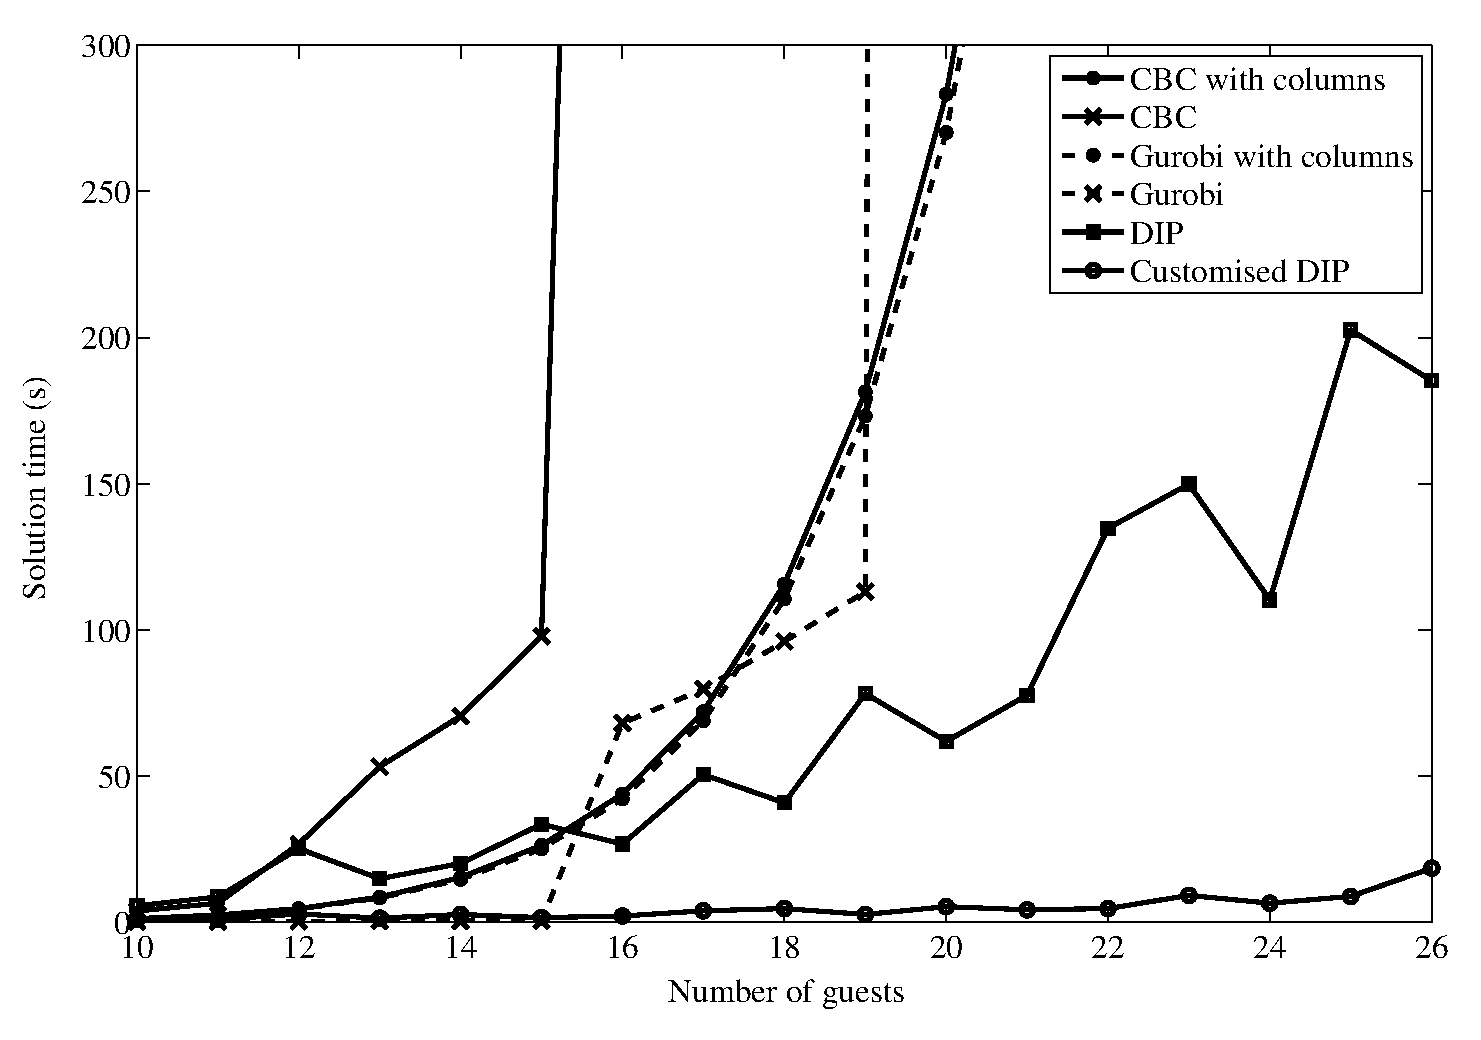
\includegraphics[scale=0.600]{img/wedbench.eps}
\caption{Comparing solver performance on the Wedding Planner problem. 
In this figure the times for generating the columns for ``CBC with columns'' and ``Gurobi with columns'' have been included in the total solve time. The time required for solving the original formulation sharply increases for both Gurobi and CBC (marked with crosses) but at different problem sizes. However the time for the column-wise formulation is similar for Gurobi and CBC. The time for DIP does not smoothly increase with problem size, but is consistently lower than Gurobi for instances with 16 or more guests.} \label{fig:compare}
\end{figure}

\section{Acknowledgments}

The authors would like to thank the authors of \ac{DIP}, Ted Ralphs and Matt Galati, for their help throughout this project and the Department of Engineering Science at the University of Auckland for their support of Qi-Shan during this research project.

\vspace*{-0.5\baselineskip}
\bibliographystyle{amsalpha}
\bibliography{master}

\end{document}



